
\documentclass[tikz,convert={convertexe={magick.exe}}]{standalone}

\begin{document}
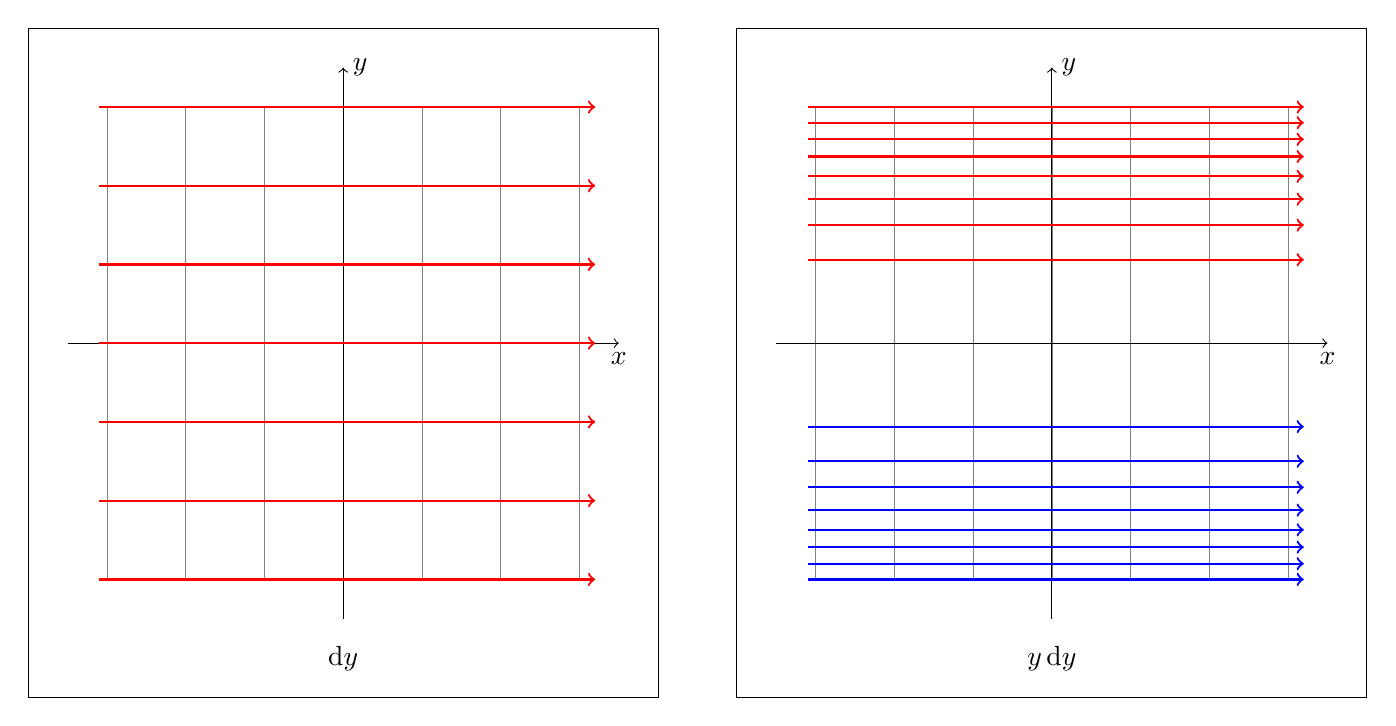
\begin{tikzpicture}

\tikzstyle atom=[circle, draw, inner sep=1.2pt, fill=red, thick]

\begin{scope}

\foreach \x in {-3,-2,...,3}
\draw[style=help lines, very thin] (\x,-3) -- (\x,3);

\draw[->] (-3.5,0)--(3.5,0) node[below] {$x$};
\draw[->] (0,-3.5)--(0,3.5) node[right] {$y$};

\draw (-4,-4.5) rectangle (4,4);
\node at (0,-4) {$\mathrm{d}y$};

\foreach \y in {-3,-2,...,3}
\draw[red, thick, ->] (-3.1,\y) -- (3.2,\y);
\end{scope}

\begin{scope}[xshift=9cm]

\foreach \x in {-3,-2,...,3}
\draw[style=help lines, very thin] (\x,-3) -- (\x,3);

\draw[->] (-3.5,0)--(3.5,0) node[below] {$x$};
\draw[->] (0,-3.5)--(0,3.5) node[right] {$y$};

\draw (-4,-4.5) rectangle (4,4);
\node at (0,-4) {$y \, \mathrm{d}y$};

\foreach \y in {1.06,1.5,1.83,2.12,2.37,2.59,2.8,3} {
\draw[red, thick, ->] (-3.1,\y) -- (3.2,\y);
\draw[blue, thick, ->] (-3.1,-\y) -- (3.2,-\y);
}
\end{scope}

\end{tikzpicture}
\end{document}